%tag:000U
%label:"art:surgeryExactTriangle"
%author:JeffHicks
%name:"the Lagrangian surgery exact triangle "
%type:"article"



Now that we have a geometric description of $L_1\#_\lambda L_2$, we discuss what object it represents in the Fukaya category. We restrict ourselves to $\dim_\RR(X)=2$ so that we may draw pictures. However, the pictures are only for intuition (and in fact the sketch of proof we give only work when $\dim(X)\geq 4$).

Let $L_0$ be some test Lagrangian, which intersects both $L_1$ and $L_2$ as in \cref{fig:roundingCorner}. If the surgery neck is chosen to lie in a neighborhood disjoint from the intersections  $L_0\cap (L_1\cup L_2)$, then these intersections are in bijection with the intersections $L_0\cap (L_1\# L_2)$. Therefore $\CF(L_0, L_1\# L_2)=\CF(L_0, L_1)[1]\oplus \CF(L_, L_2)$ as vector spaces.
%label:"fig:roundingCorner"
%author:JeffHicks
%name:"rounding corner in Polterovich surgery"
%type:"figure"
%parent:"thm_roundingCorner"
%caption:"By rounding the corner, we can compare holomorphic triangles with holomorphic strips on the surgery."


    
    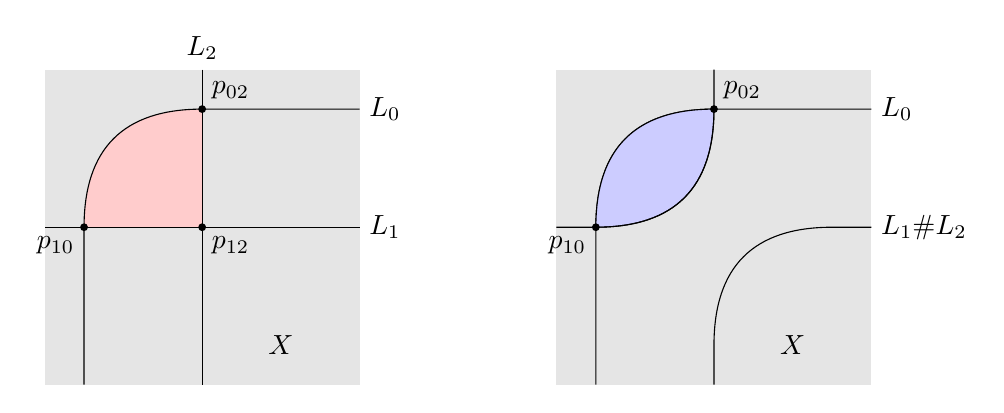
\begin{tikzpicture}\begin{scope}[]
    
    
        \fill[gray!20]  (-2,2) rectangle (2,-2);
        \fill[red!20] (0,0) .. controls (0,0.5) and (0,1) .. (0,1.5) .. controls (-1,1.5) and (-1.5,1) .. (-1.5,0) .. controls (1,0) and (0.5,0) .. (0,0);
        
        \draw (0, 2)--(0,-2);
        \draw (2,0) -- (-2,0);
        \draw (2,1.5) .. controls (1,1.5) and (0.5,1.5) .. (0,1.5) .. controls (-1,1.5) and (-1.5,1) .. (-1.5,0) .. controls (-1.5,-0.5) and (-1.5,-1.5) .. (-1.5,-2);
        
        \node[right] at (2,1.5) {$L_0$};
        \node[right] at (2,0) {$L_1$};
        \node[above] at (0,2) {$L_2$};
        \node[below right] at (0,0) {$p_{12}$};
    \node[above right] at (0,1.5) {$p_{02}$};
    \node[below left] at (-1.5,0) {$p_{10}$};
        \node[fill=black, circle, scale=.3] at (0,0) {};
        \node[fill=black, circle, scale=.3] at (0,1.5) {};
        \node[fill=black, circle, scale=.3] at (-1.5,0) {};
    \node at (1,-1.5) {$X$};
    \end{scope}
        
        
        \begin{scope}[shift={(6.5,0)}]
        
        
        \fill[gray!20]  (-2,2) rectangle (2,-2);
        \draw (2,1.5) .. controls (1,1.5) and (0.5,1.5) .. (0,1.5) .. controls (-1,1.5) and (-1.5,1) .. (-1.5,0) .. controls (-1.5,-0.5) and (-1.5,-1.5) .. (-1.5,-2);
        
        \node[right] at (2,1.5) {$L_0$};
        \node[right] at (2,0) {$L_1\#L_2$};
        
        
        \draw[fill=blue!20] (0,1.5) .. controls (0,0.5) and (-0.5,0) .. (-1.5,0) .. controls (-1.5,1) and (-1,1.5) .. (0,1.5);
        
        \draw (0,2) .. controls (0,1.5) and (0,2) .. (0,1.5) .. controls (0,0.5) and (-0.5,0) .. (-1.5,0) .. controls (-2,0) and (-2,0) .. (-2,0);
        \draw (0,-2) .. controls (0,-2) and (0,-2) .. (0,-1.5) .. controls (0,-0.5) and (0.5,0) .. (1.5,0) .. controls (2,0) and (2,0) .. (2,0);
        
        
    \node[above right] at (0,1.5) {$p_{02}$};
    \node[below left] at (-1.5,0) {$p_{10}$};
        \node[fill=black, circle, scale=.3] at (0,1.5) {};
        \node[fill=black, circle, scale=.3] at (-1.5,0) {};
    \node at (1,-1.5) {$X$};
        \end{scope}
        
        \end{tikzpicture}
 The intuition from \cite{fukaya2007lagrangian} is that there is a bijection between certain holomorphic triangles with boundary on $L_0, L_1, L_2$ which passes through the intersection point $p_{12}$, and holomorphic strips with boundary on $L_0$ and $L_1\# L_2$. Since holomorphic triangles contribute to the $\emprod^3$ structure coefficients, and strips to the differential, it is reasonable to hope that we can state a relation between $L_1, L_2,$ and $L_1\#L_2$ as objects of the Fukaya category.


First, we observe that the intersection point $p_{12}$ determines a morphism in $\hom(L_2, L_1)$. Since we've assumed that $L_1$ and $L_2$ intersect at only one point, we know that $\emprod^1(p_{12})=0$. We can therefore form the twisted complex $\cone(p_{12})$. We now provide justification for why this is isomorphic to $L_1\# L_2$.

We have already observed that for our test Lagrangian $L_0$ we had an isomorphism of vector spaces between $\hom(L_0, L_1)\oplus \hom(L_0, L_2)$ and $\hom(L_0, L_1\#_\lambda L_2)$. The differential on $\hom(L_0, L_1\#_\lambda L_2)$ comes from counting holomorphic strips, which we break into two types: those which avoid a neighborhood of the surgery neck, and those which pass through the surgery neck. 
%label:prp:stripsInLagrangianSurgery
%name:"strips with boundary on Lagrangian surgery avoiding the neck"
%type:proposition


If $\dim_\RR(X)\geq 4$, then we can choose an almost complex structure $J$ so that whenever $p_{01}, q_{01}\in L_0\cap L_1$ are intersections, and $u: [0,1]\times \RR\to X$ is a $J$ holomorphic strip, then the boundary of $u$ is disjoint from a small neighborhood of $L_1\cap L_2$. In particular, $u$ gives a $J$-holomorphic strip with boundary on $L_0, L_1\#_{p_{12}} L_2$.

The more difficult portion is to understand the strips which pass through the neck.
%label:"thm:roundingCorner"
%author:JeffHicks
%name:"rounding the corner"
%type:"theorem"
%source:"fukaya2007lagrangian"


    Let $\dim(X)\geq 4$, and $L_1, L_2$ be exact Lagrangian submanifolds which intersect transversely at a single point $p_{12}$. Let $L_0$ be another exact Lagrangian submanifold which intersects $L_1, L_2$ transversely. Then for sufficiently small surgery necks, there exists a choices of almost complex structure on $X$ for which we have a bijection between
    \begin{itemize}
        \item $J$-holomorphic strips with boundary on $L_0, L_1\# L_2$ which pass through the surgery neck;
        \item $J$-holomorphic triangles with boundary on $L_0, L_1, L_2$.
    \end{itemize}

In fact, \cite{fukaya2007lagrangian} proves the above statement in much greater generality than we state here. The condition that $\dim(X)\geq 4$ can already be seen in in \cref{fig:roundingCorner}. Observe that if we have a pseudoholomorphic triangle whose boundary passes through the point $p_{12}$ in the wrong way, that there is no corresponding pseudoholomorphic strip with boundary on $L_0$ and $L_1\# L_2$.
Ignoring the potential complications in the definition of the Fukaya category, we obtain:
%label:cor:surgeryExactTriangle
%author:JeffHicks
%name:"surgery exact Triangle"
%type:corollary
%

\begin{corollary}
    Let $\dim(X)\geq 4$, and $L_1, L_2$ be Lagrangians which intersect transversely at a single point $p_{12}$. Then $L_1\#_{\lambda} L_2$ is isomorphic to the twisted complex $(L_1[1]\oplus L_2, \emprod^2(p_{12}-)).$
\end{corollary}
